\question A certain interstellar spaceship has a circular shape (as shown in the figure below) so that it can rotate to simulate the effect of gravity. The ship has a radius of 75 m, and a mass of $800,000$ kg. In calculating the motion of the ship, you may make treat it as a large bicycle wheel (assume all of the mass is concentrated around the perimeter, and assume the thickness of the outer shell is very small compared to the radius of the ship).

\begin{center}
	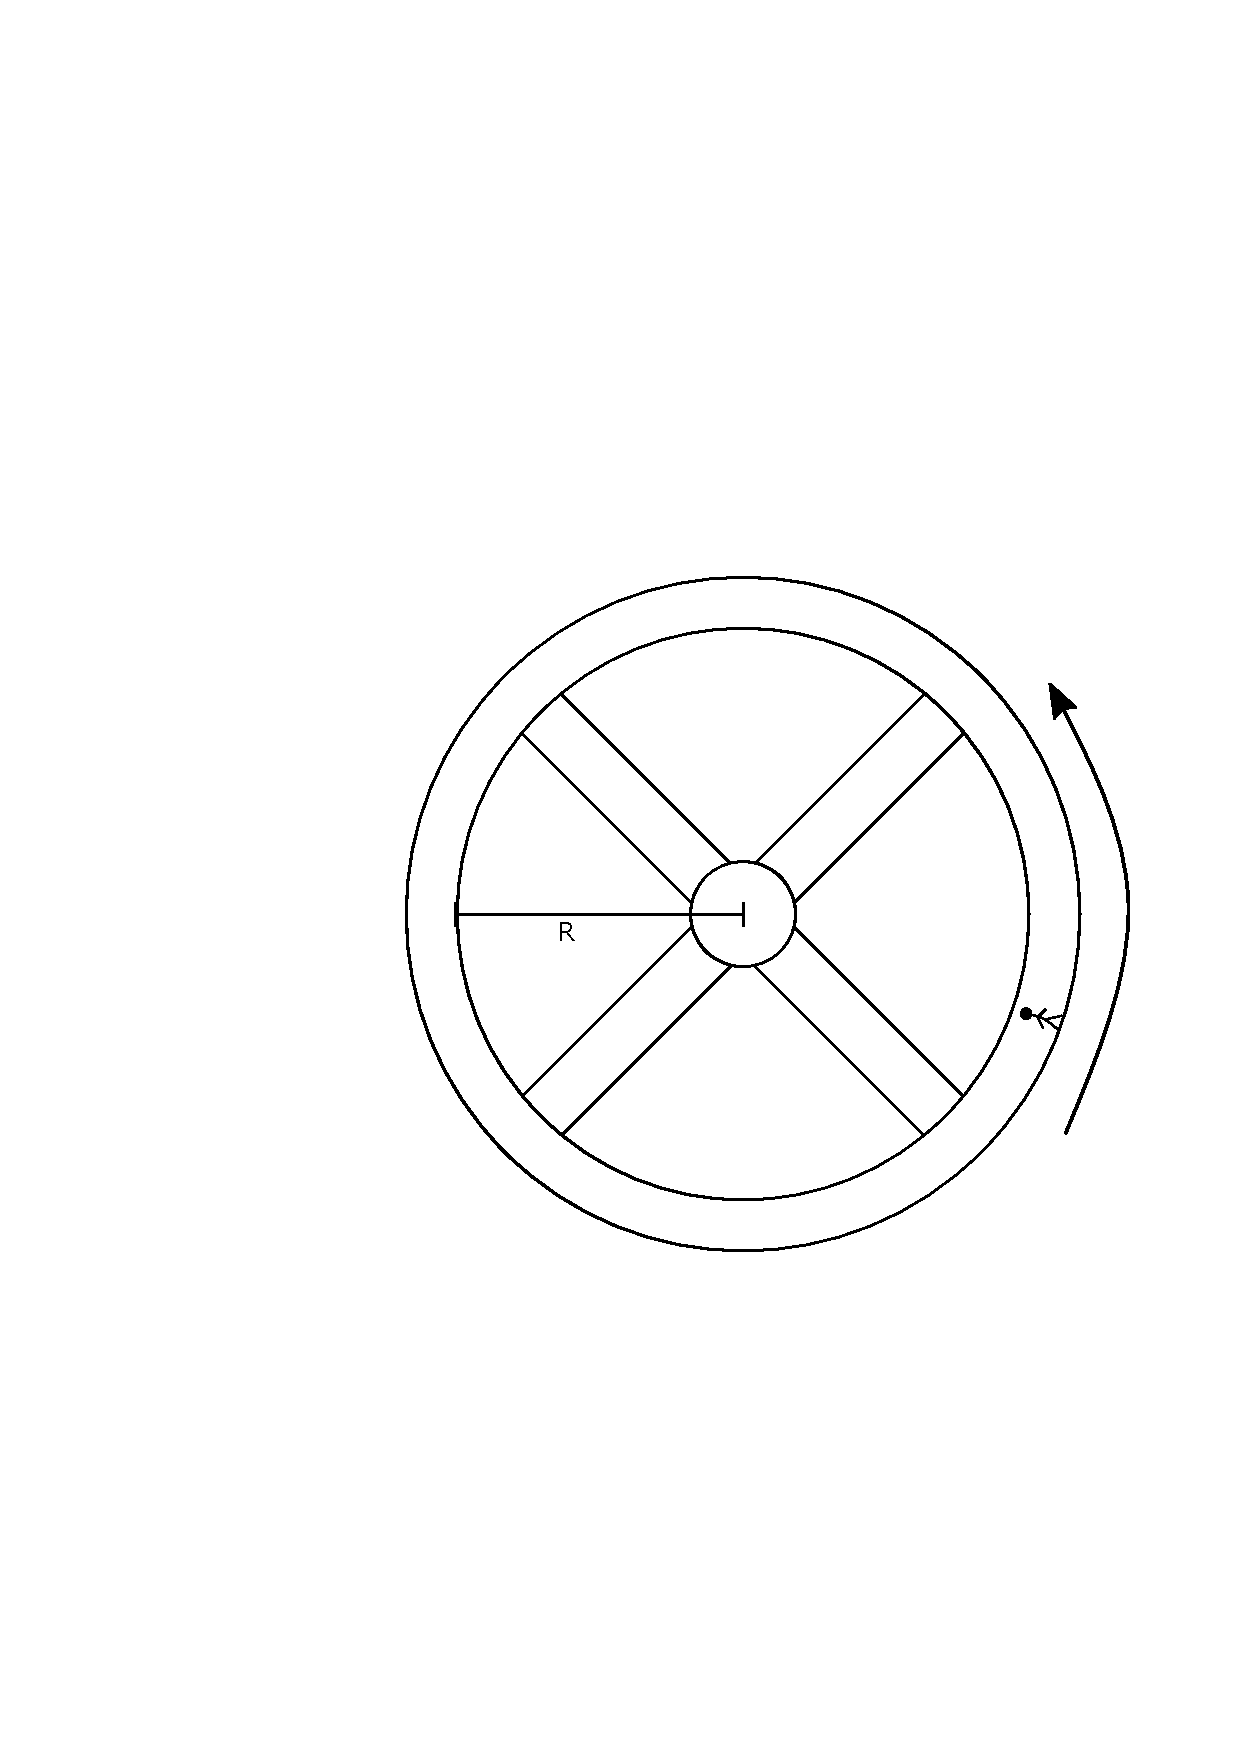
\includegraphics[width=8cm]{spaceship}
\end{center}

\begin{parts}
	\part[10] How fast must the ship spin (in rotations per second) so that the apparent weight of a person standing at the perimeter is the same as it would be on Earth?
	\vspace{4cm}
	\part[10] The ship attains this spin by firing rockets on the edge of the perimeter. How much energy must the ship use in order to achieve the rotation rate found in part (a)?
\end{parts}